%%%%%%%%%%%%%%%%%%%%%
% Documento maestro %
%%%%%%%%%%%%%%%%%%%%%
\documentclass{fime}

%%%%%%%%%%%%%%%%%%%%%%%%%%%%%%%%%%%%%%%%%%%
% Cargando paquetes y definiendo opciones %
%%%%%%%%%%%%%%%%%%%%%%%%%%%%%%%%%%%%%%%%%%%
% Aquí puedes cargar los paquetes que vas a usar. La clase
% fime ya incluye babel, inputenc, graphicx y los de la AMS.
% C1argar un paquete está a tu libertad (y responsabilidad).
\usepackage{hyperref}
\usepackage{graphicx}
\usepackage{subfig}
\usepackage{pdflscape}
\usepackage[numbers,sort&compress]{natbib}
\usepackage{float}
\usepackage{footmisc}
\usepackage{adjustbox}
\usepackage{tikz}
\usetikzlibrary{arrows, babel, shapes}
\usepackage[font=small, skip=0pt]{caption}
\setlength{\footnotesep}{0.5cm}
\setlength\footnotemargin{3pt}
\hypersetup{breaklinks=true,colorlinks=true,    linkcolor=black,citecolor=black,urlcolor=black}
\tikzstyle{decision} = [diamond, draw, fill=blue!20, text width=8em, text badly centered, node distance=3.5cm, inner sep=0pt]
\tikzstyle{block} = [rectangle, draw, fill=blue!20, text width=12em, text centered, rounded corners, minimum height=4em]
\tikzstyle{line} = [draw, -latex']
\tikzstyle{cloud} = [draw, ellipse,fill=red!20, node distance=1cm,minimum height=4em, text width=4em, text centered]
%%%%%%%%%%%%%%%%%%%%%
% Definiendo campos %
%%%%%%%%%%%%%%%%%%%%%
\def\titulo{Inventario Forestal a través de procesamiento de imágenes}
\def\autor{José Angel Ramírez Cantú}
\def\matricula{1628685}
\def\grado{Ingeniería en Tecnología de Software}
% En caso de que el grado tenga orientación o especialidad llenar el siguiente
% campo dejando un ESPACIO INICIAL, en caso contrario, dejar vacío
\def\orientacion{}
\def\fecha{Febrero 2021} % Coloca el mes con mayúscula inicial

\def\asesor{Dra. Satu Elisa Schaeffer}
\def\revisorA{Dra. Sara Elena Garza Villarreal}
\def\revisorB{Dra. Sara Verónica Rodríguez Sánchez}
% En el caso de que tu tesis sea de doctorado activa la variable cambiándola a \doctoradotrue
% y define tus otros dos revisores
\newif\ifdoctorado\doctoradofalse
\def\revisorC{Nombre del revisor C}
\def\revisorD{Nombre del revisor D}
% El visto bueno siempre va
\def\vobo{Dr. Fernando Banda Muñoz}

%%%%%%%%%%%%%%%%%%%%%%%
% Inicia el documento %
%%%%%%%%%%%%%%%%%%%%%%%
\begin{document}

\frontmatter
\pagestyle{main}

%%% Incluye PortillasM si tu tesis es de Maestría
%%% y PortillasD si es de doctorado.
% Portadas (Maestría)

\def\uanl{Universidad Autónoma de Nuevo León}
\def\fime{Facultad de Ingeniería Mecánica y Eléctrica}
\def\depg{Subdirección Académica}
\def\snnl{San Nicolás de los Garza, Nuevo León}

%%%%%%%%%%%%%%%%%%%%%%%%
% Primer portada: UANL %
%%%%%%%%%%%%%%%%%%%%%%%%
\thispagestyle{empty}

\begin{scshape}
\begin{center}
	{\Large \uanl} \\[5mm]
	{\large \fime} \\[5mm]
	{\large \depg}
	\vskip 15mm
	
\includegraphics[height=55mm]{uanl}
	\vskip 12mm
	\begin{tabular}{p{11cm}}
		\centering
		{\large \titulo}
	\end{tabular}
	\vskip 7mm
	{por}\\[7mm]
	{\large \autor}\\[7mm]
	{como requisito parcial para obtener el grado de}\\[3mm]
	\MakeUppercase{\grado}\\
	\orientacion
	\vfill
	\fecha
\end{center}
\end{scshape}

%%%%%%%%%%%%%%%%%%%%%%%%%
% Segunda portada: FIME %
%%%%%%%%%%%%%%%%%%%%%%%%%
\newpage
\thispagestyle{empty}

\begin{scshape}
\begin{center}
	{\Large \uanl} \\[5mm]
	{\large \fime} \\[5mm]
	{\large \depg}
	\vskip 16mm
	
\includegraphics[height=50mm]{fime}
	\vskip 16mm
	\begin{tabular}{p{11cm}}
		\centering
		{\large \titulo}
	\end{tabular}
	\vskip 7mm
	{por}\\[7mm]
	{\large \autor}\\[7mm]
	{como requisito parcial para obtener el grado de}\\[3mm]
	\MakeUppercase{\grado}\\
	\orientacion
	\vfill
	\fecha
\end{center}
\end{scshape}

%%%%%%%%%%%%%%%%%%%%%%%%%%%%%
% Carta del comité de tesis %
%%%%%%%%%%%%%%%%%%%%%%%%%%%%%
\newpage
\thispagestyle{empty}
\enlargethispage{5mm}

\begin{center}
{\bf \large \uanl} \\
{\bf \fime} \\
{\bf \depg}
\end{center}
\vskip 4mm

Los miembros del Comité de Tesis recomendamos que la Tesis <<\titulo>>, realizada por el alumno \autor, con número de matrícula \matricula, sea aceptada para su defensa como requisito parcial para obtener el grado de \grado\orientacion.
\ifdoctorado{\vskip 10mm}\else{\vskip 8mm}\fi

\begin{center}
El Comité de Tesis\\
\ifdoctorado{\vskip 15mm}\else{\vskip 25mm}\fi

\ifdoctorado{%%%
\begin{tabular}{p{37mm}p{21mm}p{12mm}p{21mm}p{37mm}}
	\cline{2-4}
	& \multicolumn{3}{c}{\asesor} & \\
	& \multicolumn{3}{c}{Asesor}  & \\[15mm]
	\cline{1-2} \cline{4-5}
	\multicolumn{2}{c}{\revisorA} & & \multicolumn{2}{c}{\revisorB} \\
	\multicolumn{2}{c}{Revisor}   & & \multicolumn{2}{c}{Revisor}   \\[17mm]
	\cline{1-2} \cline{4-5}
	\multicolumn{2}{c}{\revisorC} & & \multicolumn{2}{c}{\revisorD} \\
	\multicolumn{2}{c}{Revisor}   & & \multicolumn{2}{c}{Revisor}   \\[2mm]
	& \multicolumn{3}{c}{Vo. Bo.} & \\[14mm]
	\cline{2-4}
	& \multicolumn{3}{c}{\vobo}   & \\
	& \multicolumn{3}{c}{\depg}   & \\ &&&&
\end{tabular}
}\else{%%%
\begin{tabular}{p{37mm}p{21mm}p{12mm}p{21mm}p{37mm}}
	\cline{2-4}
	& \multicolumn{3}{c}{\asesor} & \\
	& \multicolumn{3}{c}{Asesora}  & \\[19mm]
	\cline{1-2} \cline{4-5}
	\multicolumn{2}{c}{\revisorA} & & \multicolumn{2}{c}{\revisorB} \\
	\multicolumn{2}{c}{Revisora}   & & \multicolumn{2}{c}{Revisora}   \\[2mm]
	& \multicolumn{3}{c}{Vo. Bo.} & \\[17mm]
	\cline{2-4}
	& \multicolumn{3}{c}{\vobo}   & \\
	& \multicolumn{3}{c}{\depg}   & \\ &&&&
\end{tabular}
}\fi%%%

\vfill

\snnl, \MakeLowercase{\fecha}

\end{center}

%%%% Dedicatoria

\thispagestyle{empty}
\vspace*{17mm}

\begin{flushright}
\begin{itshape}

Aquí puedes poner tu dedicatoria\\
si es que tienes una.\bigskip\bigskip

Si no tienes una, puedes borrar\\
la línea \verb+% Dedicatoria

\thispagestyle{empty}
\vspace*{17mm}

\begin{flushright}
\begin{itshape}

Aquí puedes poner tu dedicatoria\\
si es que tienes una.\bigskip\bigskip

Si no tienes una, puedes borrar\\
la línea \verb+% Dedicatoria

\thispagestyle{empty}
\vspace*{17mm}

\begin{flushright}
\begin{itshape}

Aquí puedes poner tu dedicatoria\\
si es que tienes una.\bigskip\bigskip

Si no tienes una, puedes borrar\\
la línea \verb+\include{Dedicatoria}+ en el\\
archivo \texttt{MiTesis.tex} pues no es obligatoria.

\end{itshape}
\end{flushright}

+ en el\\
archivo \texttt{MiTesis.tex} pues no es obligatoria.

\end{itshape}
\end{flushright}

+ en el\\
archivo \texttt{MiTesis.tex} pues no es obligatoria.

\end{itshape}
\end{flushright}



\tableofcontents
\listoffigures
\listoftables

%Agradecimientos

\chapter{Agradecimientos}
\markboth{Agradecimientos}{}

Quiero agradecer a la Dra. Elisa, por el apoyo, el conocimiento y el tiempo que invirtió durante el desarrollo de mi tesis para poder hacer una gran investigación. Al Dr. Manuel Jiménez, por el material brindado y los aportes que hizo para complementar la tesis. 

A mis padres, José Angel y Bertha Alicia, quienes siempre me motivaron a seguir adelante y son el motor de mi vida. A mis hermanas y sobrinos por su gran apoyo en todo momento, a mis abuelos Sara y José Reyes que siempre me motivaron a crecer como persona y alcanzar la meta de superarme.

Mención especial a mi abuelo Reyes (QEPD), quien en todo momento, incluso meses antes de fallecer, siempre me apoyo y espero que diera todo de mi.

%... debo mejorar esto, pero ya sé a quienes debo/quiero agradecer..
%Resumen

\chapter{Resumen}
\markboth{Resumen}{}

{\setlength{\leftskip}{10mm}
\setlength{\parindent}{-10mm}

\autor.

Candidato para obtener el grado de \grado\orientacion.

\uanl.

\fime.

Título del estudio: \textsc{\titulo}.

\noindent Número de páginas: \pageref*{lastpage}.}

%%% Comienza a llenar aquí
\paragraph{Objetivos y método de estudio:}
El objetivo de la investigación es realizar inventarios forestales por medio de las muestras recolectadas en el área del Cilantrillo y Trinidad. En la investigación se hace énfasis en utilizar la aplicación del procesamiento de imágenes para generar el inventario forestal.

\paragraph{Contribuciones y conclusiones:}
Durante la investigación se explica el funcionamiento del algoritmo que generará inventarios forestales usando el procesamiento de imágenes. Este algoritmo propone una solución eficiente y menos costosa en comparación a las técnicas manuales. 

\bigskip\noindent\begin{tabular}{lc}
\vspace*{-2mm}\hspace*{-2mm}Firma de la asesora: & \\
\cline{2-2} & \hspace*{1em}\asesor\hspace*{1em}
\end{tabular}




\mainmatter
\pagestyle{fime}

%%% Haz un documento para cada capítulo
\chapter{Introducción}
Analizar y cuantificar todo un inventario forestal puede tomar mucho tiempo, puede tender a fallar por una u otra razón, por lo que la falla humana está presente en todo momento, más sin embargo, las tecnologías que hoy en día se han desarrollado además de distintos ámbitos de la ciencia nos pueden ayudar a automatizar tareas y reducir el índice de error humano.

El \emph{aprendizaje máquina}\footnote{Campo de la inteligencia artificial que desarrolla algoritmos capaces de aprender por medio de información.} es precisamente uno de los campos de la \emph{inteligencia artificial}\footnote{Ciencia encargada de desarrollar algoritmos capaces de imitar capacidades humanas.} que nos permite resolver esta clase de problemas, ya que gracias al aprendizaje supervisado podemos usar técnicas de agrupamiento para clasificar distintas especies de árboles por medio de muestras recolectadas. En el caso del análisis de recorridos por drones, el enfoque está dirigido al área forestal dado que se podrá utilizar el aprendizaje máquina para la gestión del inventario forestal, ayudando a reducir el fallo humano y optimizando las tareas de clasificación de especies arbóreas.

Para llevar a cabo la tarea de clasificar las especies arbóreas, se recolectaron muestras de las zonas del Cilantrillo y La Trinidad en Nuevo León. Estas zonas cuentan con distintas zonas especies arbóreas como lo son: \emph{Abies, Encino y Pino}.
\newpage

\vspace*{3\baselineskip}

En las figura \ref{Zona-trinidad} se aprecia la zona de Trinidad desde distintas alturas en el mapa, el rectángulo azúl en la figura es la zona sobre la que se hizo el recorrido.

\begin{figure}[h!]
  \centering
\begin{tabular}{@{}ccc@{}}
\subfloat[Local]{\includegraphics[width=0.35\textwidth]{Cerca_t}} & 
\subfloat[Municipal]{\includegraphics[width=0.35\textwidth]{Medio_t}} &
\subfloat[Estatal]{\includegraphics[width=0.35\textwidth]{Lejos_t}}
  \end{tabular}
  \caption[Mapa de Trinidad.]{La Trinidad, Santiago, Nuevo León (25.225939, -100.1431609).}
  \label{Zona-trinidad}
\end{figure}

\hspace{15 cm}

En las figura \ref{Zona-cilantrillo} se aprecia la zona de Trinidad desde distintas alturas en el mapa, el rectángulo azúl en la figura es la zona sobre la que se hizo el recorrido.

\begin{figure}[h!]
  \centering
\begin{tabular}{@{}ccc@{}}
\subfloat[Local]{\includegraphics[width=0.35\textwidth]{Cerca_C}} & 
\subfloat[Municipal]{\includegraphics[width=0.35\textwidth]{Medio_C}} &
\subfloat[Estatal]{\includegraphics[width=0.35\textwidth]{Lejos_C}}
  \end{tabular}
  \caption[Mapa de Cilantrillo]{El Cilantrillo, Montemorelos, Nuevo León (25.3523418, -100.3463186).}
   \label{Zona-cilantrillo}
\end{figure}

\newpage

\section{Motivación}
Pese a que ya existen mecanismos de detección de objetos, muchos de ellos no funcionan con la precisión o la meta que deseamos, puesto que no se enfocan en un objetivo en particular, más sin embargo, la investigación se enfocará puramente en la detección de especies arbóreas utilizando muestras recolectadas en las zonas del Cilandrillo y Trinidad.

\section{Hipótesis}
Se sabe que el procesamiento de imágenes tiene como finalidad enfocarse en
la búsqueda de un elemento en particular, en nuestro caso las especies arbóreas; se plantea demostrar que el procesamiento de imágenes permitiría reducir tiempos de recorrido a pie y optimizar costos en cuanto a la realización de inventarios forestales por medio de técnicas tradicionales.

\section{Objetivos}
En esta sección se establece el objetivo general y los objetivos específicos sobre los que se enfoca la tesis.

\subsection{Objetivo general}
El objetivo de realizar el inventario forestal por medio del procesamiento de
imágenes tiene un propósito más práctico que técnico. El algoritmo permitiría a quienes se encarguen de analizar las zonas forestales, reducir el tiempo invertido en aplicar técnicas tradicionales por técnicas de procesamiento de imágenes.

Estas técnicas  basadas en el aprendizaje máquina, el cual permitir
generar un inventario forestal mediante el recorrido de un dron y a su vez, analizarlo por medio de la inteligencia artificial con la finalidad de indicar las cantidad de especies reconocidas sobre una zona.

\subsection{Objetivos específicos}
\begin{itemize}
\item Realizar un algoritmo capaz de detectar específicamente los árboles y su especie arbórea.
\end{itemize}

\begin{itemize}
\item El algoritmo debe extraer la información de un set de especies arbóreas, mismas que servirían como modelo para una fase posterior de detección de especies arbóreas.
\end{itemize}

\begin{itemize}
\item El algoritmo debe ser capaz de detectar por si mismo las especies encontradas en cada una de las muestras recolectadas.
\end{itemize}

\pagebreak

\section{Estructura}
En el capítulo 2 expone algunos antecedentes que han surgido a lo largo
de la historia respecto a los inventarios forestales, así como las características más importantes sobre las que trabaja el procesamiento de imágenes.

En el capítulo 3 se hace la comparación de algunos trabajos relacionados con la detección de objetos y el procesamiento de imágenes, también analiza un poco cuales son los aspectos fundamentales que se desarrollarán en la investigación.

En el capítulo 4 hace un vistazo a las muestras sobre las que se está trabajando además de la explicación de la primera fase de la investigación, el procesamiento de muestras.

En el capítulo 5, expone las fases restantes de la investigación, las cuales corresponden a el entrenamiento, la detección y la combinación respectivamente.

En el capítulo 6 discute los resultados posteriores a la ejecución del algoritmo.

Por último en el capítulo 7, se determina una conclusión respecto a la investigación desarrollada.

\chapter{Antecedentes}
Hoy en día existen diversas tecnologías que acaparan la atención por su funcionalidad y la interacción que tienen con procesos cotidianos, pero también existen tecnologías capaces de sustituir habilidades que sólo podrían ser propias de un ser humano, es por eso que en la presente investigación se está trabajando con el aprendizaje máquina y su aplicación en el análisis de zonas forestales.

Como se mencionó antes, el aprendizaje máquina hace uso de muestras para identificar las especies arbóreas según su clase, sin embargo, el proceso de etiquetar o identificar objetos por medio de aprendizaje máquina lleva por nombre \emph{clasificación de imágenes}\footnote{Es una técnica del aprendizaje máquina que consiste en identificar un objeto por medio de propiedades o características propias de un elemento.}.

El \emph{procesamiento de imágenes}\footnote{Su función es capturar y procesar por medio de imágenes la información más relevante.} analiza por medio de características como: \emph{forma, color, bordes, textura} cuando se utiliza en conjunto con el aprendizaje máquina. Sin embargo, las características dependerán en gran medida del objetivo ya que no todas las características aportan información relevante para el procesamiento y clasificación. Las características utilizadas en el análisis de especies arbóreas serán clasificadas en características locales y características globales.

\section{Antecedentes históricos}
El procesamiento de imágenes surge en el año 1920 de los primeros intentos de transmisión de imágenes por medio de un cable transatlántico usando códigos telegráficos, permitiendo la codificación de una imagen en cinco niveles de gris para posteriormente, en 1929, el ya mencionado sistema de transmisión permitía codificar a quince niveles de gris, a su vez, este sistema redujo el tiempo de transmisión de imágenes a quince minutos \citep{rf4}. 

El aprendizaje máquina surge a principios del año 1990 como un proceso para la extracción de información y modelos de predicción, esto último fue bastante utilizado por los sectores bancarios, que eran los que mayormente le sacaban un provecho a la hora de tomar decisiones \citep{rf5}. 

La \emph{visión computacional}\footnote{Técnica de la inteligencia artificial que intenta emular la capacidad visual de los humanos.} llevaba bastante más tiempo que había sido desarrollada, pero no empleada; y es que en el año 1960 es cuando la inteligencia artificial apenas se estaba desarrollando y fue cuando se planteo el como es que una computadora iba a razonar como lo haría una persona. Los problemas recaen sobre factores de innovación y procesamiento de imágenes automático. No obstante, más delante en los descriptores de características, se explicarán a detalle como es que la visión computacional hace uso de ellas \citep{rf6}.

Por otro lado, los \emph{inventarios forestales} surgen como respuesta a ciertas interrogantes como lo son el manejo sostenible de un bosque y los elementos que lo conforman. Estos se definen como sistemas de recolección de características del área sobre el que se trabaja \citep{rf7}.

\section{Descriptores de características globales}
La idea de que el color presente en las muestras recolectadas sea el único diferenciador de una especie respecto a otra es un pensamiento incorrecto debido a que además de este criterio, existen otros criterios que nos permiten apreciar e identificar las características de una especie arbórea, no obstante, estas características pueden ser útiles en otras fases de la investigación. 

\subsection{Color}
La característica de clasificación de color hace uso del \emph{histograma de color}\footnote{Cantidad de pixeles en listas de rangos de colores presentes en una imagen.}, aunque también se puede hacer uso de la \emph{estadística de canal de color}\footnote{Muestran la distribución de píxeles presentes en una imágen.} aunque en este caso, se omite la última. Los histogramas de color suelen ser utilizados por ejemplo, en motores de búsqueda de imágenes para encontrar correlaciones de distribuciones de colores similares. También pueden ser visualizados en forma de gráficas de intensidad de la distribución del valor de un \emph{pixel}\footnote{Es la unidad básica más pequeña de las imágenes.}.

\begin{figure}[h!]
  \centering
\begin{tabular}{@{}ccc@{}}
\subfloat[Muestra utilizada]{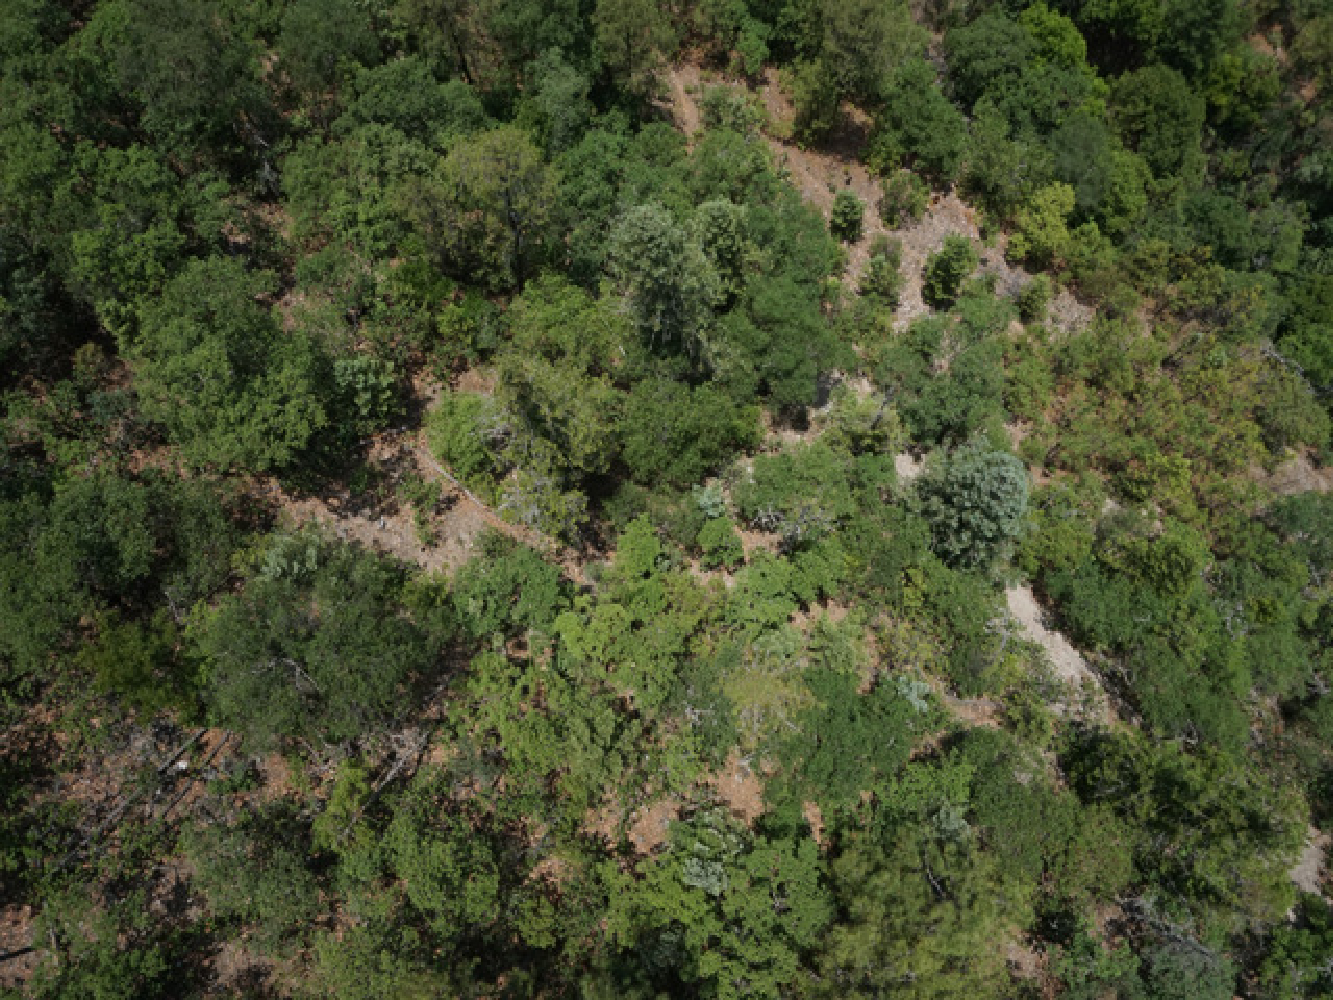
\includegraphics[width=0.45\textwidth]{DSC06100}} & 
\subfloat[Histograma generado]{\includegraphics[width=0.45\textwidth]{histograma-gen}} &
  \end{tabular}
  \caption[Histograma de color]{Histograma de color generado con las bibliotecas \texttt{matplotlib y OpenCV.}}
  \label{Histograma-generado}
\end{figure}


\subsection{Forma}
La característica de forma cuenta también con varias métricas, se hace énfasis en los \emph{momentos de una imagen}. 
Los momentos de una imagen son los pesos promedio de la intensidad de píxel sobre una imagen.  

\begin{figure}[h!]
  \centering
  \begin{minipage}[b]{0.8\textwidth}
    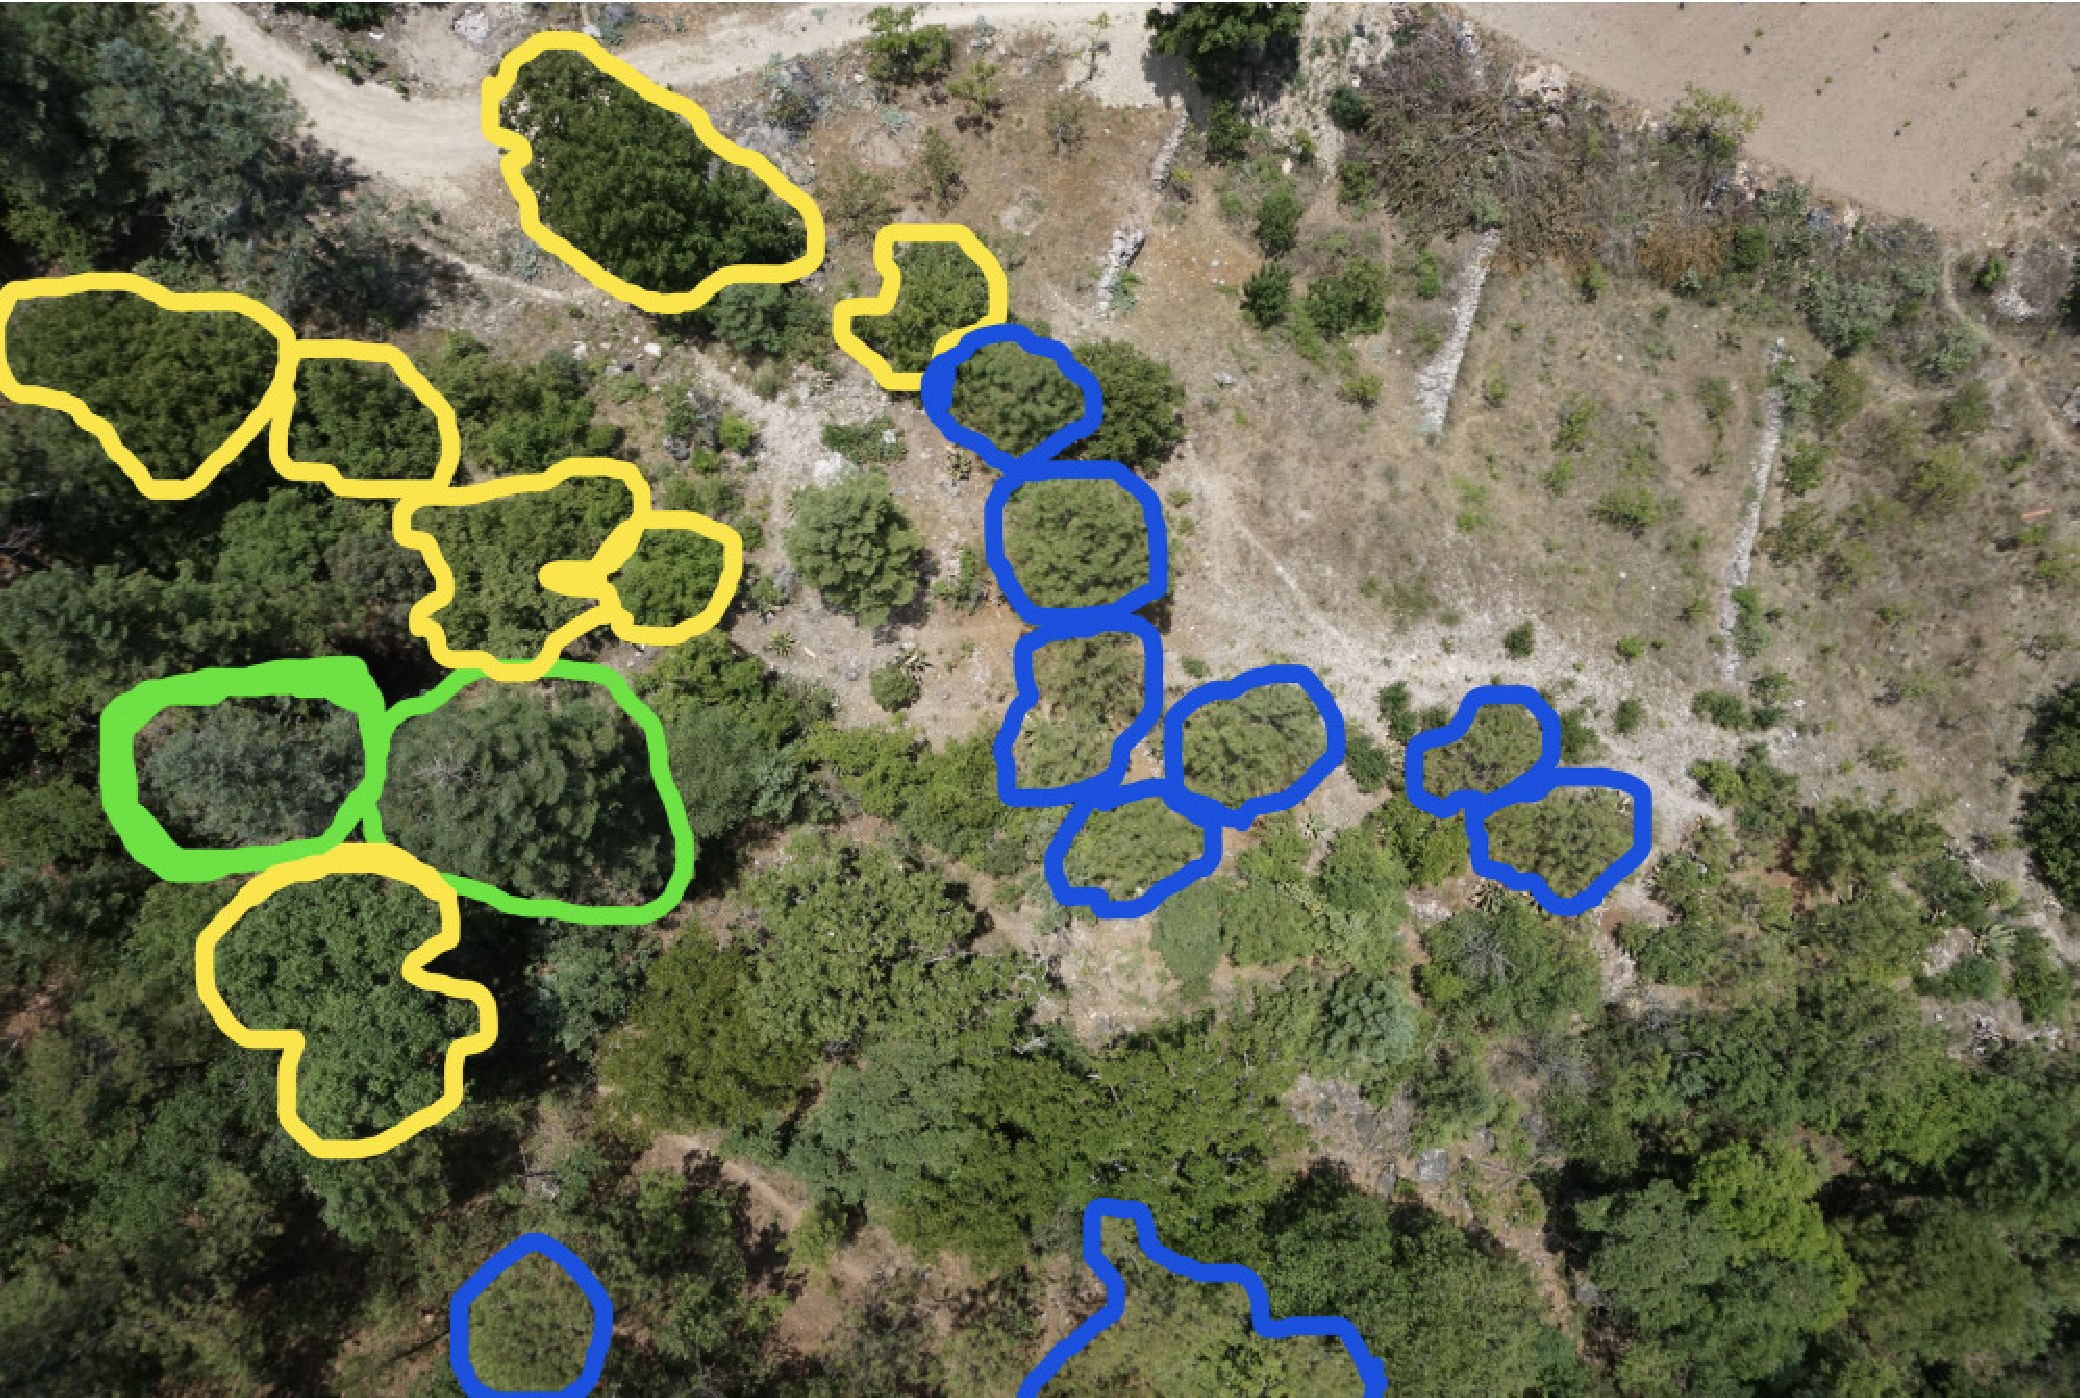
\includegraphics[width=\textwidth]{Anotaciones-ex}
    \caption[Formas de cada especie arbórea.]{Formas de cada especie arbórea (verde: Abies, azúl: Pino, amarillo: Encino).}
  \end{minipage}
\end{figure}

Por ejemplo, el canal $I$ de una imagen contiene una intensidad en los ejes $(x,y)$ dados por la ecuación $I(x,y)$ donde $I(x,y)$ hace referencia una imagen binaria donde sólo es posible tomar un valor cero o uno. En otras palabras, los momentos de una imagen son un conjunto de siete números calculados del movimiento central que son invariantes para las transformaciones de una imagen. 

\begin{equation}
\label{eq:2.1}
 M = \sum_{x}\sum_{y} I(x,y).
\end{equation}

La ecuación \ref{eq:2.1} obtiene la sumatoria de la intensidad de todos los píxeles, es decir, la sumatoria se hace con base únicamente en la intensidad de los píxeles y no con la posición dentro de una imagen.

\subsection{Textura} 
Esta característica tiene una gran relevancia dado que es de las más usadas al momento de identificar objetos en regiones de interés en fotografías aéreas, micrográficas y de satélite y en nuestro caso, al identificar las muestras de los árboles. En este caso haremos uso de la métrica de \emph{textura de Haralick}. 

La Figura 2.3 ilustra las distintas texturas que tienen los especies arbóreas en la imagen, a simple vista algunos colores denotan ser de una especie distinta si se hace un análisis minucioso, pero en este caso, la característica de textura puede ser utilizada para diferenciar entre especies arbóreas.

\begin{figure}[h!]
  \centering
  \begin{minipage}[b]{0.7\textwidth}
    \includegraphics[width=\textwidth]{textura-cil}
    \caption{Texturas en muestra del Cilantrillo}
  \end{minipage}
\end{figure}

\section{Descriptores de características locales}
Las características anteriormente mencionadas cuantifican globalmente una imagen, sin embargo, para poder determinar las características que cuantifican localmente las regiones de una imagen es necesario determinar que descriptor será el óptimo para describir los puntos de interés de una imagen completa o los puntos de interés de cierta región de la imagen. 

\begin{description}
\item[SIFT (Característica de transformación de escala invariante)]{Extra la información de una imagen para posteriormente, permita adecuarla cuando se desee compararla con diferentes muestras de un objeto o escena.}
\end{description}

\begin{description}
\item[SURF (Característica de acelerado robusto)]{Toma un vecino al rededor del punto seleccionado en la imagen y es dividido en sub-regiones para cada sub-región, la respuesta de la transformada de Wavelet es tomada y representada por esta característica.}
\end{description}
 
\begin{description}
\item[BRIEF (Características elementales  independientemente binarias robustas)]{Se enfoca en la orientación de una imagen y depende del menor numero de diferencias (puntos) a su alrededor.}
\end{description}

\begin{description}
\item[ORB (BRIEF Rotada y orientada rápida)]{Se relaciona con BRIEF debido a
que esta es una fusión de la ya mencionada con un punto detector clave rápido (FAST). Para determinar estos puntos clave rápido, se utiliza FAST y posteriormente, la medida de esquinado de Harris es aplicada para encontrar los $n$ puntos más altos. En concreto, esta característica registra la intensidad ponderada del centroide la cual está localizada en la esquina de un centro.}
\end{description}

\section{Uso de los descriptores}
Existen varias formas de utilizar los descriptores pero hay dos maneras de mezclar las características de vectores.

\paragraph{•} Para las características globales de vector, nosotros sólo concatenaremos cada característica del vector para formar a una característica global del vector simple. Este enfoque será el utilizado en el desarrollo de este algoritmo.

\paragraph{•} Para las características locales del vector también puede hacerse una combinación de las características locales y globales del vector, pero necesitaremos algo llamado \emph{modelo de la bolsa de palabras} (BOVW). Este enfoque se utiliza normalmente en constructores de vocabularios, Clustering de K-media, etc.

\paragraph{•} El \emph{escalamiento} es también otra de los descriptores utilizados en las características de los vectores, este sirve para transformar los datos de las características en rangos específicos de cero a uno, por ejemplo. Esta característica suele ser bastante usada en máquina de soporte vectorial y en el \emph{K-vecinos cercanos} (KNN) donde la distancia entre dos puntos es importante.

\paragraph{•} La \emph{normalización} es utilizada en los descriptores también, esta última es una técnica donde los valores son desplazados y re-escalados  para que puedan alcanzar un rango entre cero y uno, a esta característica también se le conoce como \emph{escalamiento mínimo-máximo}.

\chapter{Estado del arte}
En este capítulo se explica la relación de la investigación en curso con investigaciones de otros autores, la importancia de la visión computacional y su relación con los inventarios forestales, así como los apartados que se desarrollan durante la investigación.

\section{Investigaciones relacionadas}
Existen algunos trabajos que no están completamente relacionados con el objetivo de identificar especies arbóreas, pero si existen investigaciones que toman como objetivo el analizar zonas forestales.

Este artículo nos menciona como hacen uso de combinar datos para realizar inventarios forestales por medio de sistemas digitales aéreos de fotogrametría y escáneres láser. Con estas tecnologías, hacen una búsqueda buscando los tipos predominantes en una zona y con ayuda del \emph{análisis de imágenes basado en objetos} se pudo admitir la delineación automática de árboles, la clasificación de especies arbóreas y la definición de atributos estructurales a nivel de árbol. 
\newline
\break


\cite{rf1} Utiliza una gran cantidad de entradas para definir manualmente la especie, no obstante, la principal diferencia es que este trabajo no realiza por medio de visión computacional sino por técnicas tradicionales .
 
\cite{rf2} tiene como meta evaluar artículos para actualizar los inventarios de árboles en un área metropolitana. En este no se trata con inteligencia artificial como tal, pero si hacen uso de tecnologías de detección como sensores remotos que permitan evaluar correctamente y obtengan la información concreta de las zonas donde habitan  árboles.

\cite{rf3} tienen como objetivo detectar objetos además de hacer uso del umbral adaptativo, el cual es muy utilizado en la visión computacional. %El problema a solucionar en concreto como parte de este trabajo es, resolver los métodos de umbralización.

\cite{rf9} hace simulaciones para la gestión de modelos forestales que podría ser requeridos para la toma de decisiones en un sector forestal. En este artículo se hacen validaciones usando modelos generados por información de un bosque privado y un bosque estatal de Illinois, EE.UU.

\cite{rf10} hace uso de técnicas de inteligencia artificial para la identificación  de especies forestales haciendo uso de multidatos espectrales tomando como punto de partida, los vecinos más cercanos (KNN) para procesar eficientemente la información recolectada y segmentar por clusters el ambiente sobre el que se trabajó.

\pagebreak
 
\section{Comparación de trabajos}
La mayoría de los trabajos citados hacen uso de otra clase de tecnología que no tiene que ver directamente con la utilizada en nuestra investigación, más sin embargo, algunos de los aspectos clave que se presentan en nuestra investigación con respecto a las investigaciones encontradas son:

\begin{description}
\item[Inventarios forestales]{ Son aquellos que nos permiten tener un control de las especies que pueblan una zona específica.}
\end{description}

\begin{description}
\item[Análisis de imágenes]{Es una técnica bastante utilizada hoy en día por la visión computacional para extraer datos e información de imágenes.}
\end{description}

\begin{description}
\item[Visión computacional]{Este concepto está completamente relacionado con la inteligencia artificial, dado que es una  técnica del aprendizaje máquina que busca encontrar objetos emulando la capacidad humana del reconocimiento.}
\end{description}

\begin{description}
\item[Clasificación]{Es el acto de separar u ordenar bajo un criterio específico.}
\end{description}

\begin{description}
\item[Especies]{Son los distintas categorías o  clases de algún objeto en particular.}
\end{description}

\begin{description}
\item[Zonas]{Es algún sector o delimitación de territorio de algún sitio, ciudad, país.}
\end{description}

\begin{description}
\item[Detección de objetos]{Es una técnica del aprendizaje máquina que emula la capacidad humana de detectar por si sola, algún objeto por medio de la vista.}
\end{description}

\newpage

\subsection{Comparaciones}
En el cuadro \ref{tab:Comparación de trabajos frente al desarrollado}, podemos apreciar que características podemos encontrar en las investigaciones citadas anteriormente y su relación con la investigación con la que se está trabajando actualmente.\\
\renewcommand{\tablename}{Cuadro}
\begin{table}[hbt!]
	{\centering
	\caption{Comparación de trabajos frente al desarrollado}
	\begin{adjustbox}{width=\textwidth}
		\begin{tabular}{|c|c|c|c|c|}
			\hline
			Trabajo &  Inventarios forestales &  Visión Computacional & Detección de objetos\\
			\hline
			\cite{rf1} & \checkmark & $\times$ & \checkmark \\
			\hline
			\cite{rf2}&  \checkmark  &  $\times$ & $\times$  \\
			\hline
			\cite{rf3}& $\times$ & \checkmark & \checkmark  \\
			\hline	
			\cite{rf9}& \checkmark & \checkmark & \checkmark  \\
			\hline
			\cite{rf10}& $\times$ & \checkmark & \checkmark  \\
			\hline
			\cite{rf11}& $\times$ & \checkmark & \checkmark  \\
			\hline
			\cite{rf12}& \checkmark  & $\times$ & $\times$  \\
			\hline
			\cite{rf13}& \checkmark & $\times$ & $\times$  \\
			\hline
			\cite{rf14}&  $\times$ & \checkmark & $\times$   \\
			\hline
			\cite{rf15}& \checkmark & \checkmark & $\times$  \\
			\hline
			Investigación & \checkmark & \checkmark & \checkmark \\
			\hline
		\end{tabular}
	\end{adjustbox}
	\label{tab:Comparación de trabajos frente al desarrollado}}
\end{table}

\subsection{Áreas de oportunidad}
En el cuadro 3.1 se puede apreciar que características tiene la investigación que se trabaja con respecto a la de otros autores, y es que, a simple vista pudiera ser que otros trabajos tengan las mismas características o al menos casi todas, pero por lo que respecta a la investigación, la ventaja que tiene es que, además de ser un código libre para que cualquier persona pueda verlo, es que la investigación se está aplicando sobre un problema real, es decir, generar los inventarios forestales. 

\newpage
Por otro lado, también se puede apreciar que el trabajo de \cite{rf10} tiene las mismas características que nuestro trabajo pero va orientado a otro objetivo, que es tomar decisiones. Sin embargo, las herramientas descritas en el artículo no son de uso gratuito, permitiendo así, otorgar la ventaja de que la investigación sea de licencia abierta respecto a esta investigación.

En lo que respecta a las áreas de oportunidad de la investigación, podemos destacar el aprendizaje máquina (ML) y la visión computacional como herramientas clave. Primeramente, el aprendizaje máquina nos ayudará para poder entrenar un algoritmo cuyo producto será bastante relevante en el proceso de clasificación durante la investigación.

En nuestro caso, el aprendizaje máquina se encargará de extraer información clave de cada una de las muestras recolectadas de las zonas forestales, donde, mediante descriptores de características tanto globales como locales, se encargará de generar un archivo que contenga la información más relevante de las muestras.

Posteriormente, la visión computacional hará uso del archivo generado previamente por el aprendizaje máquina donde se hará cargo de clasificar cada árbol mediante una etiqueta que definirá su especie por color. Esto último no ha sido aplicado en las investigaciones encontradas puesto que tienen un enfoque nulo en hacer clasificaciones de múltiples objetos de un sólo tipo, o bien, sólo se enfocan en hacer anotaciones manuales por medio de inputs previamente establecidos y esto únicamente se enfoca en comparaciones.

El Inventario forestal es otro de los apartados importante en la investigación, dado que es uno de los enfoques en los que se el desarrollo de los algoritmos que vamos a utilizar, se estará tomando como punto de partida al momento de desarrollarse. 

Clasificación es quizás el punto más importante de la investigación debido a que, en base a esto, se estará haciendo un análisis de las muestras recolectadas previamente por los drones y posteriormente serán tratadas por los algoritmos de clasificación, haciendo uso de la visión computacional y el aprendizaje máquina, donde se estarán entrenando los modelos para posteriormente ser clasificados.


\chapter{Recolección de muestras}
Habiendo conocido las características que mejor describen a los atributos de nuestro algoritmo, podemos decir que la base de nuestro algoritmo se puede desarrollar.

La primera fase a considerar en el desarrollo de esta, sería recolectar muestras de el objeto(s) a identificar por medio del aprendizaje máquina. Si bien es necesario tener una gran cantidad de muestras para que nuestro algoritmo tenga una perspectiva más amplia de lo que se necesita reconocer, también hay que considerar que necesitamos información que contenga la menor cantidad de información no útil dado que esto podría sobre entrenar al modelo que se encargue de la clasificación.

\section{Muestras recolectadas}
Inicialmente se proporcionó un repositorio con imágenes alojado en Google Drive que contenía imágenes de las zonas donde se realizó el recorrido del dron, más específicamente \textbf{Cilandrillo} y \textbf{Trinidad}.

\begin{figure}
 \centering
\includegraphics[scale=0.5]{Cilandrillo}
\caption{Muestras de la zona de Cilandrillo}
\end{figure}

\begin{figure}
 \centering
\includegraphics[scale=0.5]{Trinidad}
\caption{Muestras de la zona de Trinidad}
\end{figure}

\subsection{Análisis de muestras}
Como se mencionó anteriormente, es importante recolectar una gran cantidad de muestras para entrenar bien el modelo, por lo que para la zona del Cilandrillo se recolectaron 277 muestras y para la zona de Trinidad se recolectaron 270 muestras. Esta cantidad de muestras es suficiente para entrenar bien nuestro modelo que será capaz de reconocer los distintos tipos de árbol, más sin embargo, en cada imagen se puede apreciar información que no es útil y puede sobre entrenar el modelo, perjudicando de forma que este detecte más en concreto, el suelo como un tipo de árbol.

La información de cada muestra es analizada píxel por píxel, por lo que a simple vista podemos percatarnos de que clase de información tiene cada muestra, pero el analizar cada una de ellas llevaría demasiado tiempo, por lo que, podemos concluir que habrá pixeles dentro de ellas que no sean útiles. 

En los casos de la figura \textbf{4.3} y \textbf{4.4} mostramos un pequeño ejemplo de cómo se verían las muestras que nos son de utilidad y destacando que en el siguiente capitulo apreciaremos el procedimiento realizado para poder obtener muestras útiles.

\begin{figure}[b]
  \centering
  \begin{minipage}[b]{0.4\textwidth}
    \includegraphics[width=\textwidth]{DSC06080}
    \caption{Muestra no útil}
  \end{minipage}
  \hfill
  \begin{minipage}[b]{0.4\textwidth}
    \includegraphics[width=\textwidth]{DSC06080-sf}
    \caption{Muestra útil}
  \end{minipage}
\end{figure}

\newpage

\subsection{Información no útil}
En cada una de las muestras recolectadas está presente el suelo ya que es una imagen capturada por un drone, sin embargo, el suelo forma parte de la información que necesitamos remover de las muestras para no sobre entrenar a nuestro modelo de reconocimiento.

Para efectos prácticos, se declararon los colores de las especies arbóreas, esto con el fin de decirle a nuestro algoritmo que información no debe remover de las muestras. A su vez tenemos que declarar que la información será reemplazada con pixeles transparentes. Cabe destacar que nuestras imágenes no cuentan con un canal alpha, mismo que es necesario para llevar a cabo nuestro procedimiento de reemplazar la información, por lo que tenemos que convertir cada muestra primero, a un formato .png para que la muestra admita este canal. Después se tendrá que convertir la muestra a un canal \textbf{RGBA} (Red Gray Blue Alpha).

 Una vez que la muestra tenga el canal alpha recorreríamos todos los pixeles de la imagen con el fin de encontrar y asignar a una variable, todos los pixeles que no correspondan con los colores de los árboles y posteriormente, ir descartando de estos pixeles con el fin de guardar la muestra con la información útil como se muestra en la figura \textbf{2.5}.

\begin{figure} [!b]
	\centering
	\begin{minipage}[b]{0.5\textwidth}
		\includegraphics[width=\textwidth]{DSC06080-sf}
		\caption{Resultado de remover píxeles}
	\end{minipage}
\end{figure}

\break

\section{Fase de procesamiento de muestras}
Una vez recolectadas las muestras con información relevante, se procede a  entrenar a el modelo con esa información para que sea en fases posteriores este sea capaz de entender y clasificar donde estén presentes las especies arbóreas almacenadas en el modelo. La forma de organizar cada muestra para un correcto entrenamiento es mediante la separación de cada especie por su color correspondiente, es decir, separando las especies de color azul en una carpeta, los verdes y los amarillos en su carpeta correspondiente consecuentemente.

\subsection{Recortando muestras por islas}
Primeramente hay reconocer las secciones o partes de la muestra que son de nuestro interés, en este caso, vamos a estar trabajando como antes con los colores, específicamente los de cada especie de árbol. En el caso de todas las muestras, tenemos tres colores: [verde, amarillo, azul, azul claro, rosa, púrpura, verde limón, amarillo oscuro, azul oscuro, gris oscuro, gris claro]. Estos colores nos van a indicar que colores tienen una anotación valida para recortar.


\begin{figure}[H]
  \centering
  \begin{minipage}[b]{0.5\textwidth}
        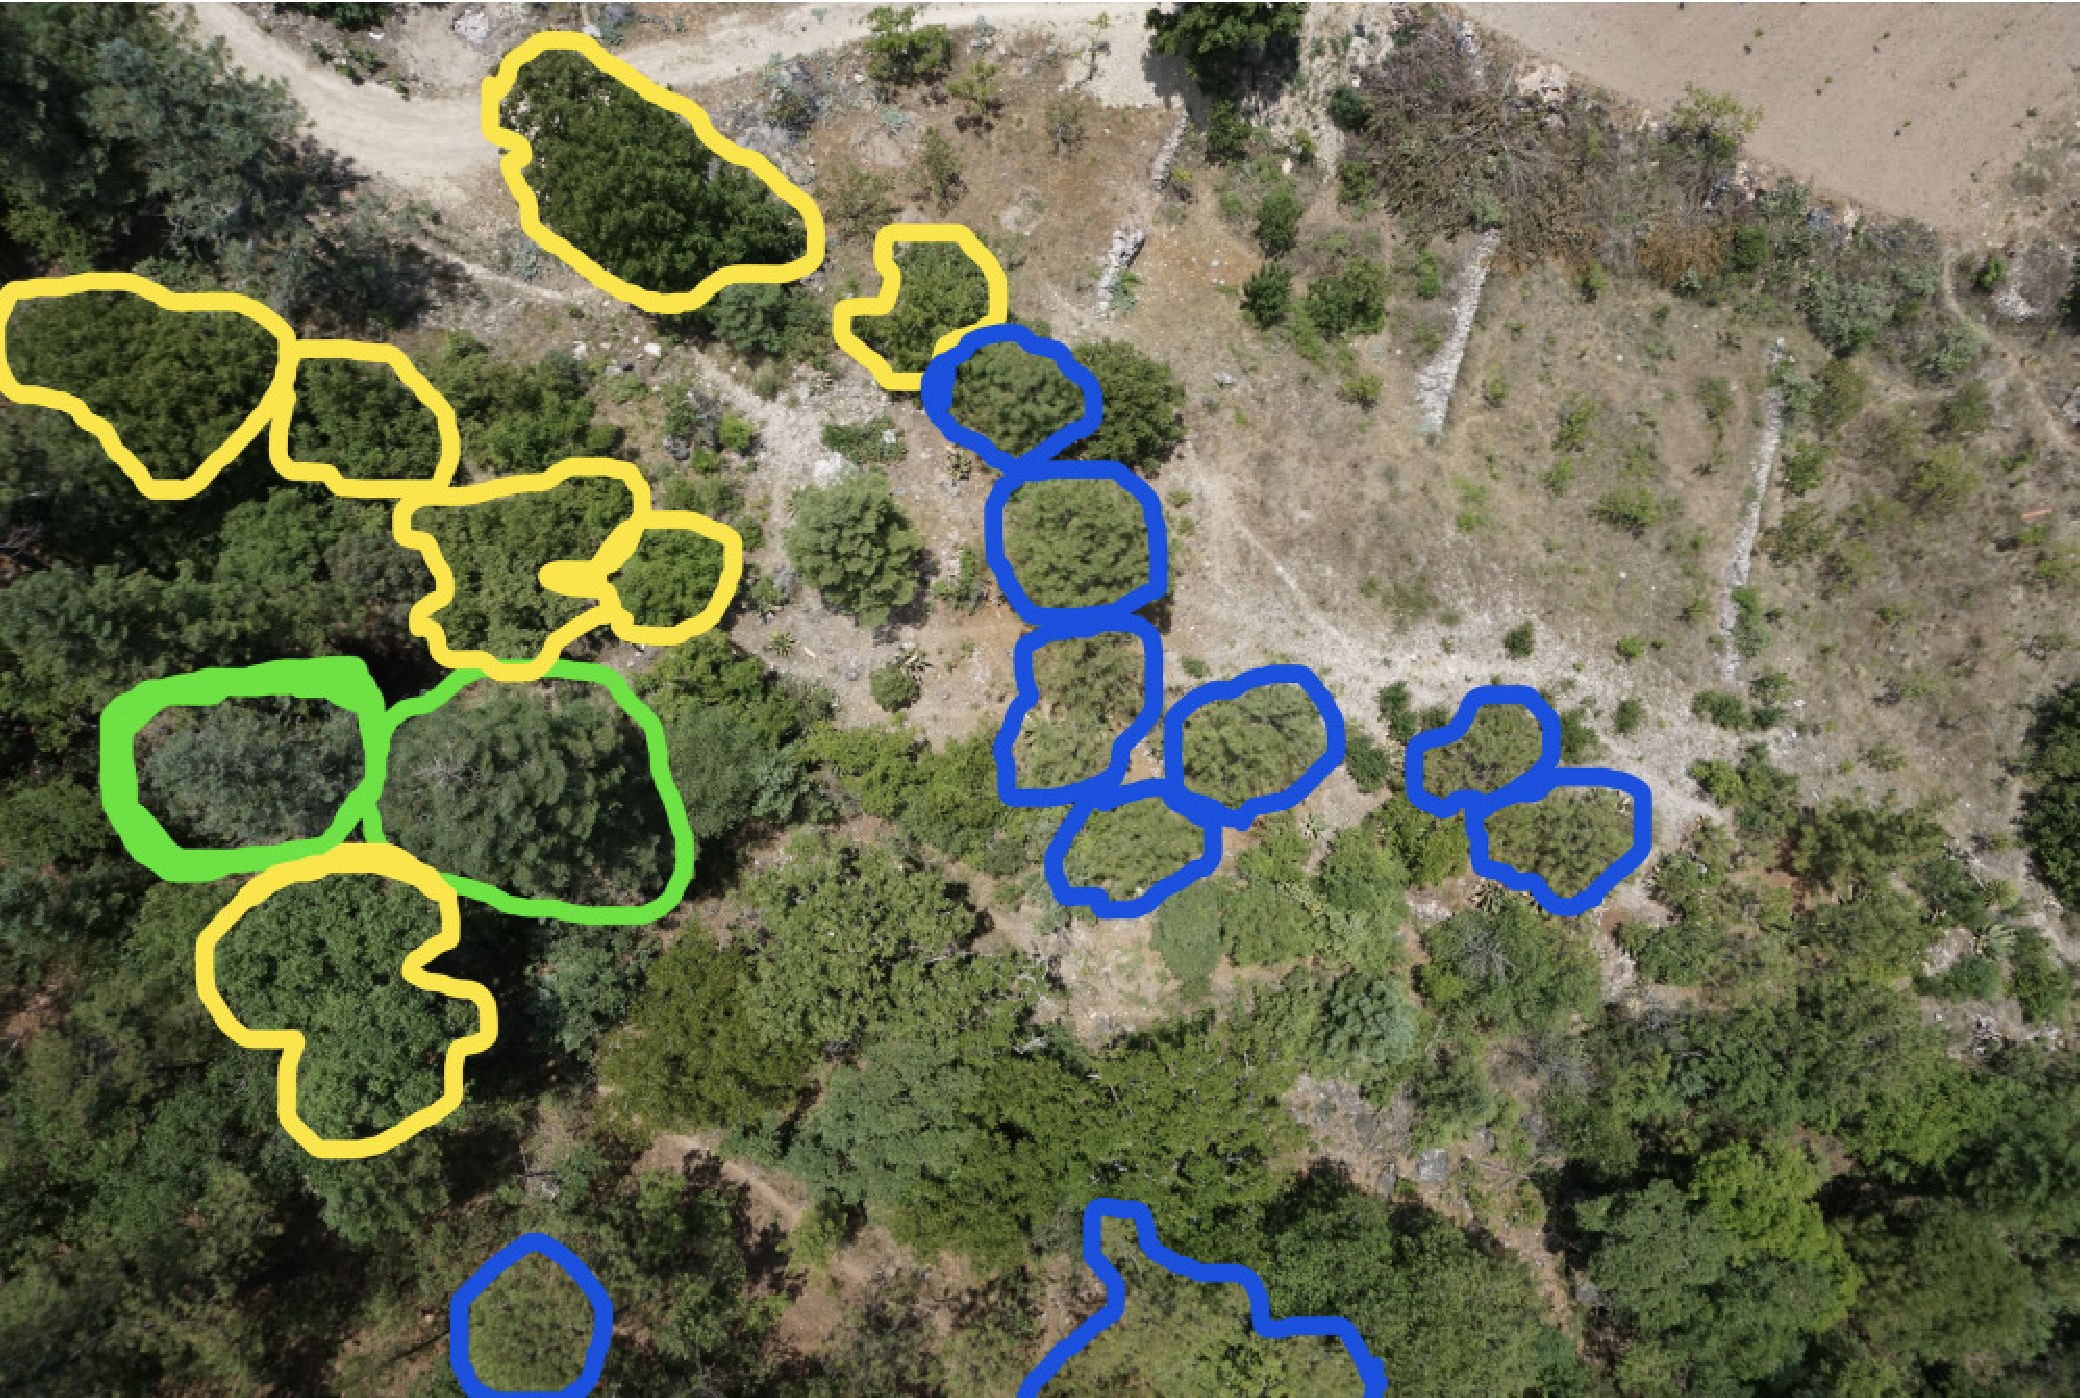
\includegraphics[width=\textwidth]{Anotaciones-ex}
    \caption{Muestra con anotaciones}
  \end{minipage}
\end{figure}

En nuestro caso podemos apreciar la figura \textbf{4.6} que tiene secciones delimitadas por colores, por lo que iremos recorriendo la muestra por pixeles hasta encontrar la zona que esté dentro del rango de colores previamente establecido.

La idea de hacer recortes de las anotaciones por colores es de agilizar el procesamiento a la hora de entrenar nuestro modelo con todas las muestras. Cada muestra a su vez, tendrá un porcentaje de admisión que permitirán indicar si la anotación cumple o no con los criterios establecidos.

Ya con las muestras de colores obtenidas, se procede a separar por islas de acuerdo al color que este establecido. Se separarán por color verde, amarillo y azul, cada color en una carpeta distinta para tener mayor control de las islas capturadas.

\begin{figure}[H]
  \centering
  \begin{minipage}[b]{0.5\textwidth}
        \includegraphics[width=\textwidth]{muestras_color}
    \caption{Isla separada por color}
  \end{minipage}
\end{figure}

En la figura \textbf{4.7} se puede apreciar un ejemplo de como quedan las islas separadas por color, por lo que ahora tendríamos que hacer recortes de cada una de las islas con el fin de obtener únicamente recortes interiores que nos provean más detalle de cada zona recortada y posteriormente, sean procesadas de mejor forma por el modelo que estaremos entrenando. \\

\break

Una vez se tienen las islas, se hacen recortes interiores dentro de cada una de ellas. Los rectángulos generados por medio de las islas tienen un tamaño fijo de 150 x 150, donde a su vez, cada 25 pixeles, se va buscando rectángulos con un porcentaje de 0.005 píxeles no transparentes.


\begin{figure}[h]
  \centering
  \begin{minipage}[b]{0.7\textwidth}
        \includegraphics[width=\textwidth]{rectangulo_isla_ex}
    \caption{Rectángulo del interior de una isla}
  \end{minipage}
\end{figure}


En la figura \textbf{4.8} se puede apreciar uno de los rectángulos generados por medio de una muestra. Estos no sólo se quedan como tal fijos, sino que se rotan en tres orientaciones, 90, 180 y 270, permitiendo que el conjunto de datos generado esté compuesto por distintos ángulos de la muestra y permita tener mejor perspectiva de lo que se va a utilizar.

\break

\section{Validaciones}

Previo a realizar el entrenamiento con el set generado por parte del algoritmo de entrenamiento, se realiza una validación que hará uso de las muestras separadas por color sólo que esta será mostrada de forma distinta.

En el caso de las validaciones, únicamente se realiza con el propósito de reconocer que modelo de entrenamiento es el que mejor funciona a la hora de realizar la clasificación y sea el óptimo en este caso. \\


\begin{figure}[h]
 \centering
\includegraphics{comparacion_algoritmos}
\caption[Comparación de algoritmos]{Comparación de algoritmos al momento de realizar las validaciones}
\end{figure}

\break

\chapter{Desarrollo de solución}

Posterior a obtener las muestras separada por islas, la fase siguiente consistiría en entrenar un modelo que nos permita hacer el reconocimiento de las especies arbóreas. Lo anteriormente mencionado se haría obteniendo la información más importante usando a las muestras que contienen a las islas sin información que pueda llegar a sobrescribir el modelo.

Cabe destacar que el modelo nos servirá en gran medida debido a que etiquetará las especies de árboles almacenadas con las características previamente mencionadas (textura, forma y color) en las muestras originales en la fase final.

\section{Fase de entrenamiento}
Originalmente conocemos las distintas especies arbóreas que forman parte de nuestra colección o set de imágenes, pero al momento de clasificar, nuestro algoritmo estará recorriendo la carpeta que contiene las muestras útiles, por lo que primero indicamos por medio de un arreglo, el conjunto de carpetas a buscar con los rectángulos que se generaron a partir de las muestras, es decir, buscar en las carpetas: \textbf{green, blue y yellow}. \\

Es necesario declarar durante la fase del entrenamiento las clases a utilizar y el tamaño de muestras para posteriormente generar un set que nos sea de utilidad. En nuestro caso, declaramos un tamaño de 250 muestras por clase (color) y seguido se irán recorriendo el arreglo de carpetas para ir buscando en cada muestra las características mencionadas en el \textbf{capítulo 2, sección 2.3} donde mencionamos a las características globales.

Al ir recorriendo las muestras, las procesamos primero guardándolas en un variable local que determinarán el tamaño de estas para posteriormente, utilizarlas al extraer las características globales. Cuando se tiene almacenada la información extraída de las muestras, se añade a un vector de características globales el cual será guardado dentro del un conjunto de datos que contiene la información de cada una de las muestras y posteriormente, utilizado al momento de clasificar las especies de árbol. 

\section{Fase de detección}
Esta fase es la más importante de todas debido a que utilizamos los modelos generados a partir de la fase de entrenamiento. En esta fase se utilizan las características globales de extracción de características previamente comentadas en el capítulo \textbf{capítulo 2, sección 2.3} donde hacemos uso del modelo de clasificador forestal aleatorio \footnotemark{\textbf{Random Forest Classifier}}, donde tenemos que poner un valor estimado de arboles por cada muestra donde se vaya a probar el modelo, en nuestro caso utilizaremos como valor de 200. Posteriormente tenemos que definir que utilizar la información de los modelos de características utilizadas y las etiquetas de muestras generadas a partir de ello también. 
\footnotetext{Random Forest Classifier: Es un clasificador de multiples decisiones que funciona en conjunto.}
\\

\begin{figure}[H]
  \centering
  \begin{minipage}[b]{0.8\textwidth}
        \includegraphics[width=\textwidth]{resultado_clasificacion}
    \caption{Detectando árboles en una muestra}
  \end{minipage}
\end{figure}

Tal y como se muestra en la figura \textbf{5.1}  podemos notar como una especie es detectada según su color a lo largo de una muestra, no obstante, podemos destacar que cada especie también tiene encima de su cuadro un nombre distinto debido a que las especies arbóreas con las que se trabaja son: \textbf{Abies, Pino y Encino}. 

\section{Fase de combinación}
La fase de combinación trabaja indirectamente con las muestras para poder ver los resultados en una muestra con su contenido original. Para realizar una comparación, primero necesitamos obtener una muestra del directorio de muestras original donde se pueda apreciar la información no útil en ella, posteriormente se necesita obtener la muestra con las especies arbóreas detectadas en ella (producto de la fase de detección).\\ 

El proceso de combinarlas consta en tomar la información del directorio original y asignarlo como base, luego la información de las muestras con las especies detectadas es incrustado encima de la muestra original, asegurándonos que esta no contenga pixeles transparentes para evitar ensuciar la muestra original.

\begin{figure}[H]
  \centering
  \begin{minipage}[b]{0.8\textwidth}
        \includegraphics[width=\textwidth]{muestra_combinada}
    \caption{Combinación de detección y una muestra original}
  \end{minipage}
\end{figure}

Respecto a la figura \textbf{5.2} podemos destacar que la muestra original sirve como base y la muestra que contiene las especies arbóreas detectadas como mascara para poder combinar ambas capas. El objetivo de comparar las muestras generadas respecto a una muestra original es que podemos comparar cuantas especies acertaron contra las muestras con anotaciones manuales hechas por los expertos en especies.

\break


En las siguientes figuras mostraremos un poco como es que se puede percibir la diferencia entre una anotación realizada por el aprendizaje máquina a partir del modelo de datos previamente generado y la muestra con anotación hecha por un experto en el tema. \\

\begin{figure}[H]
  \centering
  \begin{minipage}[b]{0.4\textwidth}
    \includegraphics[width=\textwidth]{muestra_combinada}
    \caption{Anotaciones del aprendizaje máquina}
  \end{minipage}
  \hfill
  \begin{minipage}[b]{0.4\textwidth}
    \includegraphics[width=\textwidth]{muestra_experto}
    \caption{Anotaciones expertos}
  \end{minipage}
\end{figure}

En el caso de la figura \textbf{5.3} las anotaciones generadas a partir del aprendizaje máquina pueden contener anotaciones que no están en las anotaciones manuales pero no significa que estén incorrectas, sino que dadas las instancias otorgadas de rectángulos (green, blue, yellow) el conjunto de datos determinó que existe alguna especie en el rectángulo insertado sobre la muestra. En contra parte, la figura \textbf{5.4} nos deja ver que las anotaciones realizadas por los expertos determinan que en la figura de color marcada existe una especie.

\break

\chapter{Resultados}
Después de clasificar todas las muestras que pasaron por las fases de entrenamiento, detección y combinación, tenemos un resultado preliminar que nos indica cuantas especies fueron detectadas en la fase de detección, mismo que se discutirá en este capítulo.


Los resultados de la fase de detección serán presentandos en la tabla siguiente:

\begin{figure}[H]
  \centering
  \begin{minipage}[b]{0.5\textwidth}
        \includegraphics[width=\textwidth]{Result_detection}
    \caption{Número de especies detectadas}
  \end{minipage}
\end{figure}

La tabla 6.1 nos muestra la cantidad de especies detectadas a lo largo de la fase de detección, por lo que se puede discutir el número obtenido. A simple vista podemos notar que el número de abies nos da a entender que esa especie es predominante en las zonas del Cilandrillo y Trinidad. Posteriormente los números de la especie Pino y Encino nos muestran, en su respectivo orden, que tan predominantes son.

\section{Experimentación}
Tal y como se mostró en la sección de validaciones (Capítulo 4.3), hubo un porque detrás del hacerlo de tal manera y esto fue por la elección del algoritmo que se iba a encargar de ejecutar la detección.


\begin{figure}[H]
  \centering
  \begin{minipage}[b]{0.8\textwidth}
        \includegraphics[width=\textwidth]{algm}
    \caption{Resultado de validación}
  \end{minipage}
\end{figure}


Todas las pruebas y algoritmos fueron ejecutados en una laptop con las siguientes especificaciones:

\begin{table}[H]
	{\centering
		\begin{tabular}{|c|c|c|}
			\hline
			SO & Windows 10 x64\\
			\hline
			Procesador & Intel Core i5-7300HQ\\
			\hline
			Ram & 8 GB RAM DDR4 2133 MHz\\
			\hline
		\end{tabular}
	\caption{Especificaciones técnicas del equipo de cómputo}
	\label{tab:Especificaciones técnicas del PC}
	}
\end{table}

\break

\section{Discusión de resultados}
Tal y como se mostró en el cuadro \ref{tab:Especificaciones técnicas del PC}, el algoritmo que mejor rendimiento tiene a la hora de hacer nuestra detección es el algoritmo clasificador de bosques aleatorios el cual nos da un score mucho menor en comparación a otros al momento de realizar el entrenamiento del clasificador.

Cabe recalcar que el rendimiento de este algoritmo también puede variar en relación con el procesamiento de la imagen. Esto último quiere decir que si nuestra imagen es demasiado grande, el tiempo de procesado será mayor por la cantidad de pixeles a remover y sustituir. 
No obstante, los parámetros que se agregaron para poder tener un criterio de clasificación solamente son valores muestra con el fin de abarcar la mayor cantidad de información posible y a su vez, tener un algoritmo de detección preciso.

Respecto a la ejecución de los algoritmos, es cierto que puede llegar a ser confuso el ejecutarlos si no se tiene un contexto previo de para que sirve cada uno, por eso previamente se comentaron en capítulos anteriores, que hace cada parte del algoritmo. En cuanto a limitaciones, estos pueden ser llegar a ser ejecutados en cualquier sistema operativo que permita el uso del lenguaje de programación python 3 y a su vez, las distintas bibliotecas que son necesarias para la ejecución de los scripts que componen al algoritmo.


\chapter{Conclusiones}
Después de haber obtenido los resultados del algoritmo podemos concluir algunas cosas respecto a las zonas analizadas, una de ellas es que evidentemente existe una especie predominante en ambas zonas, \textbf{Abies}, la cual en la tabla 6.1 nos dio un valor de 15567, un resultado bastante superior al de las otras especies arbóreas.

Otra de las cosas que se pudo concluir al aunar los resultados fue que el proceso de detección no hubiese sido posible de no ser removido el suelo en la fase previa al entrenamiento, esto debido a que el suelo provoca que nuestro modelo de entrenamiento hubiera sido cargado con información no útil. Con esto podemos inferir que el algoritmo hubiera clasificado de alguna forma en forma de especie las partes que contienen suelo dentro de cada muestra, haciendo que nuestro algoritmo no clasificara correctamente.

Por último y no menos importante, el tiempo de detección de muestras. Este fue la fase más tardadas de todas no sólo por el hecho de que había muchas muestras, sino que al analizar cada muestra se hacía un seguimiento de píxel por píxel para verificar el color alpha de este en la fase de seguimiento y posteriormente removerlo de la muestra, en la fase de detección, se verificaba que este no contuviera el color transparente para omitirlo y recorrer los pixeles o información útil.


\appendix
%%% Haz un documento para cada apéndice
%%\chapter{Este es un apéndice}

\section{Citas bibliográficas}

En princicpio tienes total libertad de incluir tu bibliografía con el entorno {\tt thebibliography} nativo de \LaTeX{} o mediante la herramienta \textsc{Bib}\TeX. En caso de que optes por esto último (recomendado), puedes usar alguno de los archivos {\tt mighelbib.bst} o {\tt mighelnat.bst} incluidos en el paquete {\tt Tesis-FIME}, pues sus diseños están basados en el estilo bibliográfico estándar del español, además de que armoniza con el estilo de tesis provisto por {\tt fime.cls}.

El estilo bibliográfico {\tt mighelbib} es numérico, es decir cita con un número entre corchetes, por ejemplo una cita \verb+\cite{Dan82}+ genera una etiqueta del tipo [13], mientras que el estilo {\tt mighelnat} es tipo autor-año y requiere que el paquete {\tt natbib} sea cargado (sin opciones) para su correcto funcionamiento, cita con el apellido del autor y el año, por ejemplo una cita \verb+\citet{Dan82}+ genera una etiqueta del tipo Dantzig (1982), mientras que una cita \verb+\citep{Dan82}+ genera una etiqueta del tipo (Dantzig, 1982).

Como muestra del estilo, unas citas: un libro clásico de programación lineal \cite{Baz04} y un documento histórico \cite{Dan82}. Para saber un poco más del uso de \textsc{Bib}\TeX, se puede leer \cite{Mat11}.

\section{Comillas}

El objetivo de esta sección era provocar otra página para que se vea el encabezado. Pero aprovechamos para decir que la clase {\tt fime.cls} carga el paquete {\tt babel} con la opción {\tt spanish}, por lo que cambiará automáticamente los dobles signos $<<$ y $>>$ por << y >>. Estas comillas angulares son las correctas en el idioma español, y son las que se usan en la clase {\tt fime.cls}, por lo que se sugiere sean las usadas en el texto cada que quieras <<entrecomillar>> algo.



\backmatter
\pagestyle{main}

%%% Aquí va la bibliografía, puedes usar el entorno de LaTeX (thebibliography)
%%% o la herramienta BibTeX. En caso de que optes por BibTeX, puedes usar
%%% alguno de los archivos de estilo (mighelbib.bst o mighelnat.bst) incluidos
%%% en el paquete, cuyos diseños armonizan con el diseño de tesis provisto por
%%% fime.cls. Para muestra, basta un botón:
\bibliographystyle{mighelnat}
\bibliography{MiBiblio}

\label{lastpage}
%Autobiografia

\chapter*{Resumen autobiográfico}
\thispagestyle{empty}

\begin{center}
\autor

Candidato para obtener el grado de\\
\grado\\
\orientacion\bigskip

\uanl\\
\fime\bigskip

Tesis:\\
\textsc{\large\titulo}
\end{center}\bigskip

%Aquí va tu historia
Nací el 26 de Febrero de 1997, en la ciudad de Monterrey, Nuevo León, soy el menor de tres hermanos de José Angel Ramírez Gallegos y Bertha Alicia Cantú Tamez. Actualmente trabajo como Android Developer en Linkaform, sin embargo, me apasiona trabajar en proyectos de Inteligencia Artificial y Visión Computacional, siendo estas dos últimas, el propósito de mi trabajo de titulación para el grado de Ingeniero en Tecnologías de Software.



\end{document}
